%!TEX program = xelatex
% 完整编译: xelatex -> bibtex -> xelatex -> xelatex
\documentclass[lang=cn,11pt,a4paper,cite=authoryear]{elegantpaper}




% 本文档命令
\usepackage{array}
\usepackage[final]{pdfpages}
\usepackage{graphicx}
\usepackage{float}
\newcommand{\ccr}[1]{\makecell{{\color{#1}\rule{1cm}{1cm}}}}

\begin{document}

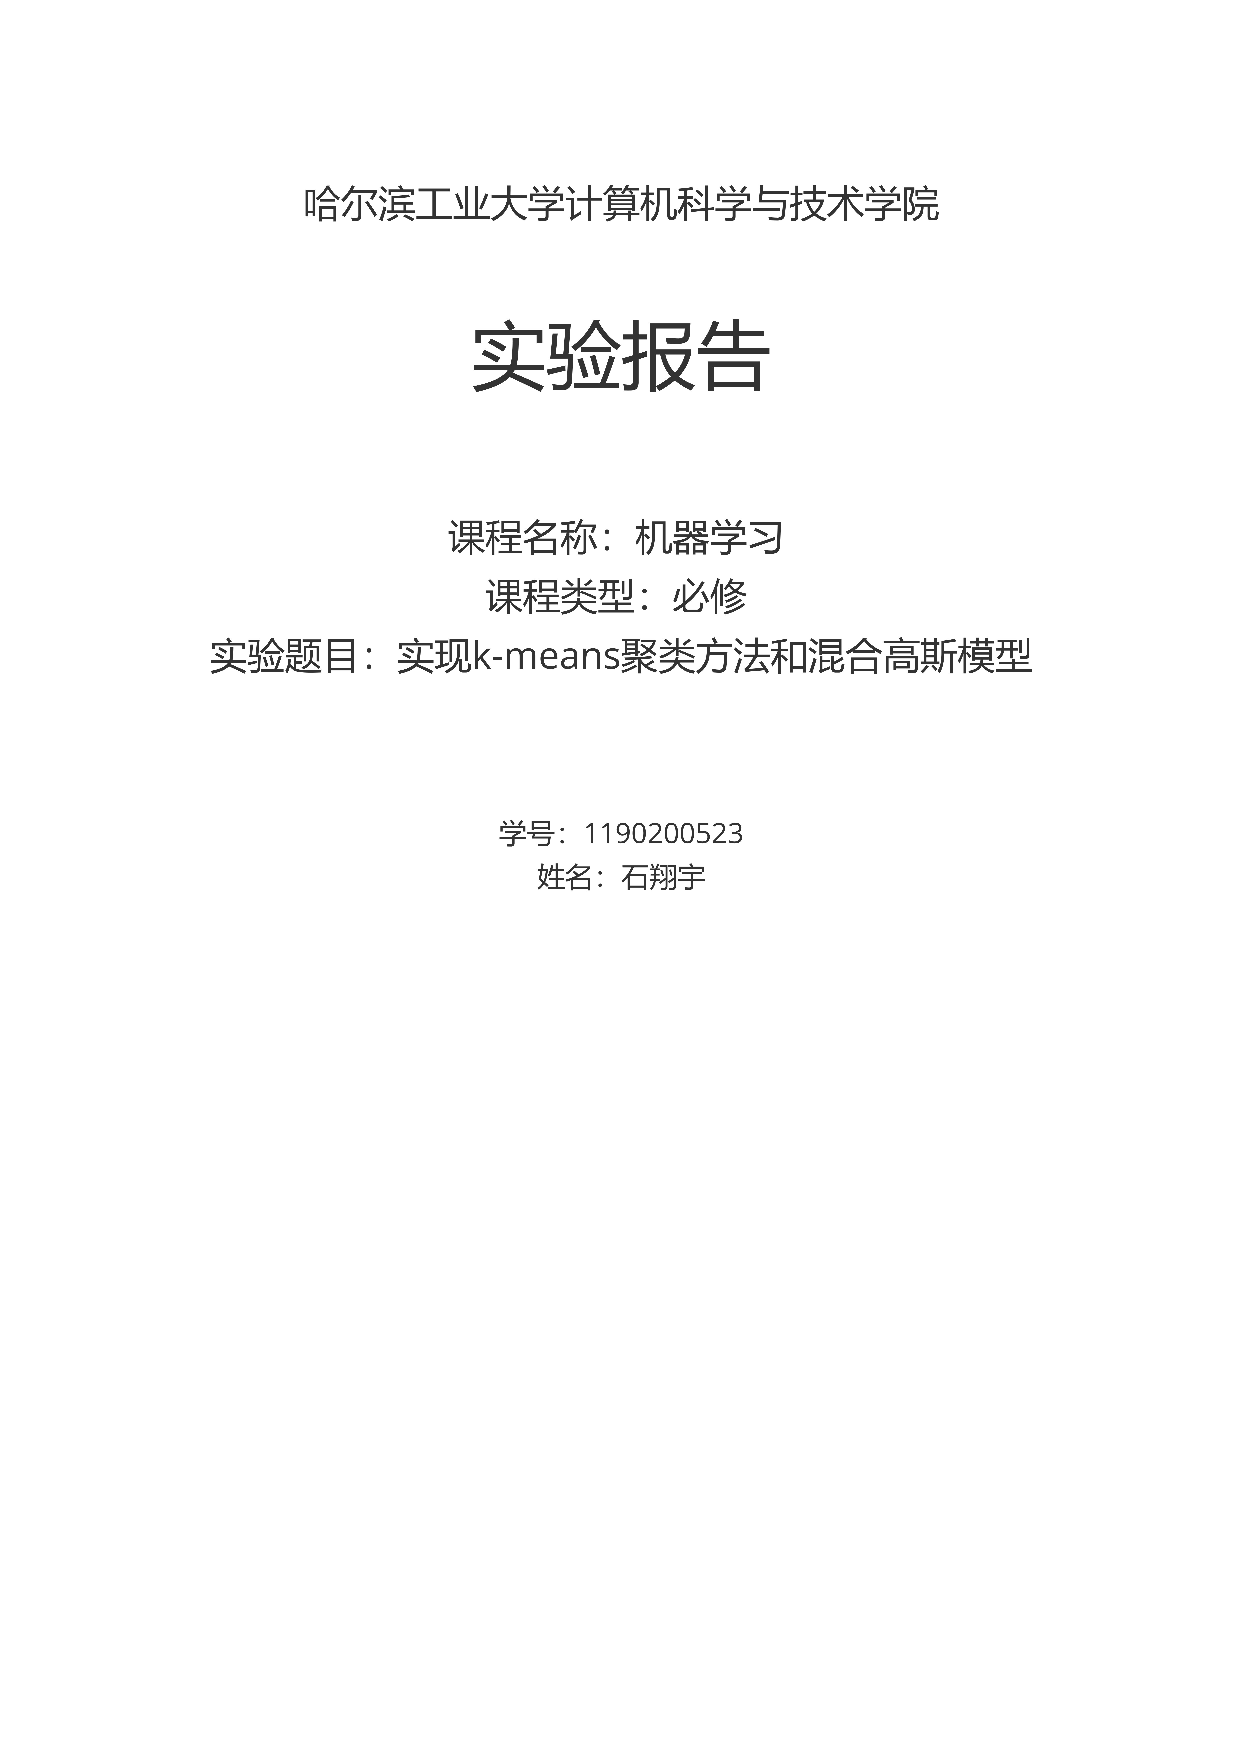
\includepdf{images/cover.pdf} 
\newpage

\section{实验目的}

实现一个k-means算法和混合高斯模型,并且用EM算法估计模型中的参数。

\section{实验要求及实验环境}

\subsection{实验要求}

\paragraph{测试}

用高斯分布产生k个高斯分布的数据(不同均值和方差),其中参数自己设定。

\begin{enumerate}
	\item 用k-means聚类,测试效果;
	\item 用混合高斯模型和你实现的EM算法估计参数,看看每次迭代后似然值变化情况,考察EM算法是否可以获得正确的结果(与你设定的结果比较)。
\end{enumerate}

\paragraph{应用}

可以UCI上找一个简单问题数据,用你实现的GMM进行聚类。

\subsection{实验环境}

Windows 11 + Python 3.7.8

\section{设计思想}

\subsection{k-means算法}

给定$n$个样本的集合$X=\{x_1, x_2,\dots,x_n\}$,$x_i\in \mathbb{R} ^m$,k-means聚类的目标是将$n$个样本分到$k$个不同的类或簇中(假设$k<n$)。$k$个类$G_1,G_2, \dots,G_k$形成对集合$X$的划分,其中$G_i\cap G_j=\emptyset$,$\bigcup\limits_{i=1}^kG_i=X$。用$C$表示划分,一个划分对应着一个聚类结果。

k-means算法通过损失函数的最小化选取最优的划分$C^*$。

首先,我们将样本之间的距离$d(x_i, x_j)$定义为欧氏距离平方
\begin{equation}
\begin{aligned}
	d(x_i,x_j)=&\sum_{k=1}^m(x_{ik}-x_{jk})^2 \\
	=&\|x_i-x_j\|^2
\end{aligned}
\end{equation}
我们定义损失函数$W(C)$为
\begin{equation}
W(C)=\sum_{l=1}^k\sum_{C(i)=l}\|x_i-\bar{x}_l\|^2
\end{equation}
其中,$\bar{x}_l=\frac{1}{n_l}\sum\limits_{C(i)=l}x_i$ ,$n_l=\sum\limits_{i=1}^nI(C(i)=l)$。

则k-means算法就是求解最优化问题
\begin{equation}
\begin{aligned}
	C^*=&arg\min_CW(C) \\
	=&arg\min_C\sum_{l=1}^k\sum_{C(i)=l}\|x_i-\bar{x}_l\|^2
\end{aligned}
\end{equation}
k-means算法是一个迭代的过程。首先,对于给定的中心值$(m_1,m_2,\dots,m_k)$,将每个样本指派到与其最近的中心$m_l$的类$G_l$中,得到聚类结果,使得目标函数极小化
\begin{equation}
\min_{m_1,\dots,m_k}=\sum_{l=1}^k\sum_{C(i)=l}\|x_i-m_l\|^2
\end{equation}
然后,对于每个包含$n_l$个样本的类$G_l$,更新其均值$m_l$
\begin{equation}
m_l=\frac{1}{n_l}\sum_{C(i)=l}x_i
\end{equation}
其中,$l=1, 2, \dots, k$。

重复上述两个步骤,直到$W(C)$结果小于阈值。

\subsection{高斯混合模型(GMM)}

高斯混合模型是指具有如下形式的概率分布模型:
\begin{equation}
P(y|\theta)=\sum_{k=1}^K\alpha_k\phi(y|\theta_k)
\end{equation}
其中,$\alpha_k\ge0$是系数,满足$\sum\limits_{k=1}^K\alpha_k=1$;$\phi(y|\theta_k)$是高斯分布密度,$\theta_k=(\mu_k,\sigma_k^2)$,$\phi(y|\theta_k)=\frac{1}{\sqrt{2\pi}\sigma_k}\exp(-\frac{(y-\mu_k)^2}{2\sigma_k^2})$。

现有观测数据$y=\{y_1,y_2,\dots,y_N\}$由高斯混合模型生成,
\begin{equation}
P(y|\theta)=\sum_{k=1}^K\alpha_k\phi(y|\theta_k)
\end{equation}
其中,$\theta=(\alpha_1,\alpha_2,\dots,\alpha_K;\theta_1,\theta_2,\dots,\theta_k)$。我们将用EM算法估计高斯混合概率模型的参数$\theta$。

我们定义隐变量0-1随机变量$\gamma_{jk}$为
\begin{equation}
\begin{aligned}
	&\gamma_{j k}= \begin{cases}1, & \text { 第 } j \text { 个观测来自第 } k \text { 个分模型 } \\
		0, & \text { 否则 }\end{cases} \\
	&j=1,2, \cdots, N ; \quad k=1,2, \cdots, K
\end{aligned}
\end{equation}
那么完全数据为
\begin{equation}
(y_j,\gamma_{j1},\gamma_{j2},\dots,\gamma_{jK}),  \quad j=1,2,\dots,N
\end{equation}
则似然函数为
\begin{equation}
\begin{aligned}
	P(y,\gamma|\theta)=&\prod_{j=1}^NP(y_j,\gamma_{j1},\gamma_{j2},\dots,\gamma_{jK}|\theta)\\
	=&\prod_{k=1}^K\prod_{j=1}^N[\alpha_k\phi(y_j|\theta_k)]^{\gamma_{jk}}\\
	=&\prod_{k=1}^K\alpha_k^{n_k}\prod_{j=1}^N[\phi(y_j|\theta_k)]^{\gamma_{jk}}\\
	=&\prod_{k=1}^K\alpha_k^{n_k}\prod_{j=1}^N[\frac{1}{\sqrt{2\pi}\sigma_k}\exp(-\frac{(y-\mu_k)^2}{2\sigma_k^2})]^{\gamma_{jk}}\\
\end{aligned}
\end{equation}
其中,$n_k=\sum\limits_{j=1}^N\gamma_{jk}$,$\sum\limits_{k=1}^Kn_k=N$。

则对数似然函数为
\begin{equation}
\log P(y,\gamma|\theta)=\sum_{k=1}^K\{n_k\log \alpha_k+\sum_{j=1}^N\gamma_{jk}[\log(\frac{1}{\sqrt{2\pi}})-\log\sigma_k-\frac{1}{2\sigma_k^2}(y-\mu_k)^2]\}
\end{equation}
EM算法的E步要求我们确定Q函数
\begin{equation}
\begin{aligned}
	Q(\theta,\theta^{(i)})=&E[\log P(y,\gamma|\theta)]\\
	=&E\{\sum_{k=1}^K\{n_k\log \alpha_k+\sum_{j=1}^N\gamma_{jk}[\log(\frac{1}{\sqrt{2\pi}})-\log\sigma_k-\frac{1}{2\sigma_k^2}(y-\mu_k)^2]\}\}\\
	=&\sum_{k=1}^K\{\sum\limits_{j=1}^N(E\gamma_{jk})\log \alpha_k+\sum_{j=1}^N(E\gamma_{jk})[\log(\frac{1}{\sqrt{2\pi}})-\log\sigma_k-\frac{1}{2\sigma_k^2}(y-\mu_k)^2]\}\\
\end{aligned}
\end{equation}
这里需要计算$E(\gamma_{jk}|y,\theta)$,记为$\hat{\gamma}_{jk}$:
\begin{equation}
\begin{aligned}
	\hat{\gamma}_{jk}=&E(\gamma_{jk}|y_j,\theta)=P(\gamma_{jk}=1|y_j,\theta)\\
	=&\frac{P(\gamma_{jk}=1,y_j|\theta)}{\sum\limits_{k=1}^KP(\gamma_{jk}=1,y_j|\theta)}\\
	=&\frac{P(y_j|\gamma_{jk}=1,\theta)P(\gamma_{jk}=1|\theta)}{\sum\limits_{k=1}^KP(y_j|\gamma_{jk}=1,\theta)P(\gamma_{jk}=1|\theta)}\\
	=&\frac{\alpha_k\phi(y_j|\theta_k)}{\sum\limits_{k=1}^K\alpha_k\phi(y_j|\theta_k)}, \quad j=1,2,\dots,N; \quad k=1,2,\dots,K
\end{aligned}
\label{eq:1}
\end{equation}
将$\hat{\gamma}_{jk}=E\gamma_{jk}$和$n_k=\sum\limits_{j=1}^NE\gamma_{jk}$代入式 \ref{eq:1} 得
\begin{equation}
Q(\theta,\theta^{(i)})=\sum_{k=1}^K\{n_k\log \alpha_k+\sum_{j=1}^N\hat{\gamma}_{jk}[\log(\frac{1}{\sqrt{2\pi}})-\log\sigma_k-\frac{1}{2\sigma_k^2}(y-\mu_k)^2]\}
\label{eq:2}
\end{equation}
EM算法的M步是要求得函数$Q(\theta,\theta^{(i)})$对$\theta$的极大值,即
\begin{equation}
\theta^{(i+1)}=\arg\max_\theta Q(\theta,\theta^{(i)})
\end{equation}
将式 \ref{eq:2} 分别对$\mu_k$和$\sigma_k^2$求偏导并令其为$0$,可得
\begin{equation}
\begin{aligned}
	\frac{\partial Q}{\mu_k} =& \sum_{j=1}^N[\hat{\gamma}_{jk}\frac{1}{\sigma^2_k}(y-\mu_k)]=0\\
	\sum_{j=1}^N(\hat{\gamma}_{jk}y)=&\sum_{j=1}^N(\hat{\gamma}_{jk}\mu_k)\\
	\sum_{j=1}^N(\hat{\gamma}_{jk}y)=&\mu_k\sum_{j=1}^N\hat{\gamma}_{jk}\\
	\mu_k=&\frac{\sum_{j=1}^N(\hat{\gamma}_{jk}y)}{\sum_{j=1}^N\hat{\gamma}_{jk}}, \quad k=1,2,\dots,K
\end{aligned}
\end{equation}

\begin{equation}
\begin{aligned}
	\frac{\partial Q}{\sigma^2_k} =& \sum_{j=1}^N[\hat{\gamma}_{jk}(-\frac{1}{2\sigma_k^2}+\frac{1}{2\sigma_k^4}(y-\mu_k)^2)]=0\\
	\sum_{j=1}^N[\hat{\gamma}_{jk}\frac{1}{\sigma_k^2}(y-\mu_k)^2]=&\sum_{j=1}^N\hat{\gamma}_{jk}\\
	\frac{1}{\sigma_k^2}\sum_{j=1}^N[\hat{\gamma}_{jk}(y-\mu_k)^2]=&\sum_{j=1}^N\hat{\gamma}_{jk}\\
	\sigma_k^2=&\frac{\sum_{j=1}^N[\hat{\gamma}_{jk}(y-\mu_k)^2]}{\sum_{j=1}^N\hat{\gamma}_{jk}}, \quad k=1,2,\dots,K
\end{aligned}
\end{equation}

对于$\hat{\alpha}_k$,需满足$\sum\limits_{k=1}^K\alpha_k=1$,则构造拉格朗日多项式:
\begin{equation}
Q'=\sum_{k=1}^K\{n_k\log \alpha_k+\sum_{j=1}^N\hat{\gamma}_{jk}[\log(\frac{1}{\sqrt{2\pi}})-\log\sigma_k-\frac{1}{2\sigma_k^2}(y-\mu_k)^2]\}+\lambda(\sum\limits_{k=1}^K\alpha_k-1)
\label{eq:3}
\end{equation}
将式 \ref{eq:3} 对$\alpha_k$求导并令导数为$0$得
\begin{equation}
\begin{aligned}
	\frac{\partial Q'}{\partial \alpha_k}=&\frac{n_k}{\alpha_k}+\lambda=0\\
	n_k+\lambda \alpha_k=&0\\
	\sum_{k=1}^Kn_k+\sum_{k=1}^K\lambda \alpha_k=&0\\
	N+\lambda=&0\\
	\lambda=&-N\\
	\alpha_k=&\frac{n_k}{N}=\frac{\sum_{j=1}^N\hat{\gamma}_{jk}}{N}, \quad k=1,2,\dots,K
\end{aligned}
\end{equation}
重复以上计算,直到对数似然值不再有明显的变化为止。

\section{实验结果分析}

\subsection{生成数据}
我们将类别数$k$设置为$3$,均值分别为$(2,7)$、$(6,2)$和$(8,7)$,协方差矩阵分别为$[[1, 0], [0, 2]]$、$[[2, 0], [0, 1]]$和$[[1, 0], [0, 1]]$,每个类别的数目设置为$150$,生成数据,结果如\figref{fig:mllab31}所示。

\begin{figure}[H]
	\centering
	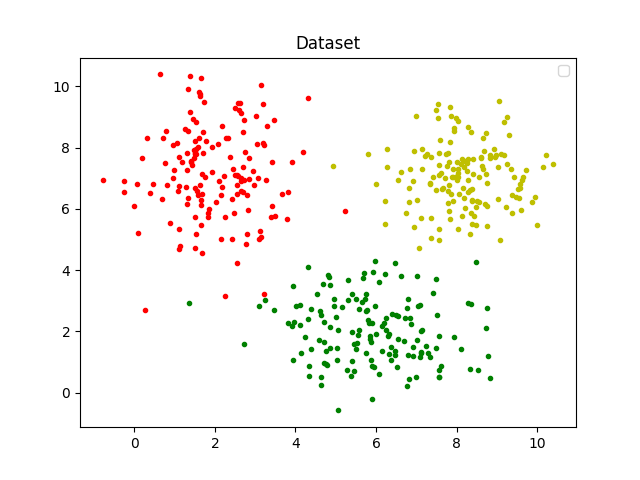
\includegraphics[width=0.7\linewidth]{images/ml_lab3_1.png}
	\caption{}
	\label{fig:mllab31}
\end{figure}


\subsection{k-means算法}

我们数据的每个类别的数目设置为$200$,其他参数不变,生成数据。我们将k-means算法的最大轮数设置为$100$轮,停止策略的系数设置为$10^{-7}$,实验结果如\figref{fig:mllab32}所示。

\begin{figure}[h]
	\centering
	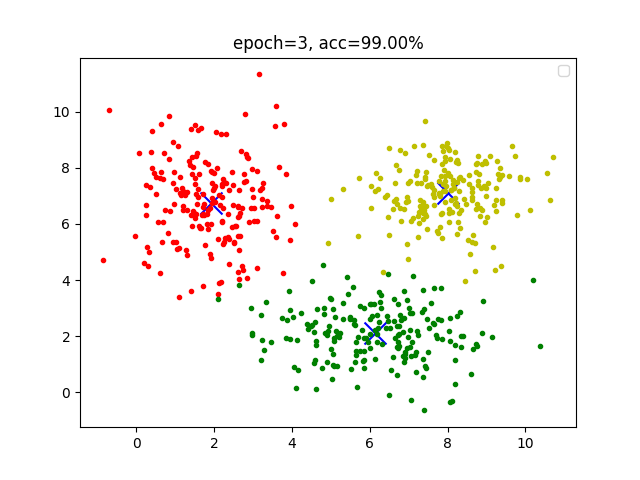
\includegraphics[width=0.7\linewidth]{images/ml_lab3_2.png}
	\caption{}
	\label{fig:mllab32}
\end{figure}

可以看到,在完成$3$轮迭代之后k-means算法收敛,得到最佳的中心点,预测准确率为$99.00\%$。k-means算法收敛速度较快,准确率也比较高。


\subsection{GMM算法}

我们数据的每个类别的数目设置为$200$,其他参数不变,生成数据。我们将GMM算法的最大轮数设置为$100$轮,停止策略的系数设置为$10^{-7}$,实验结果如\figref{fig:mllab33}所示。

\begin{figure}[h]
	\centering
	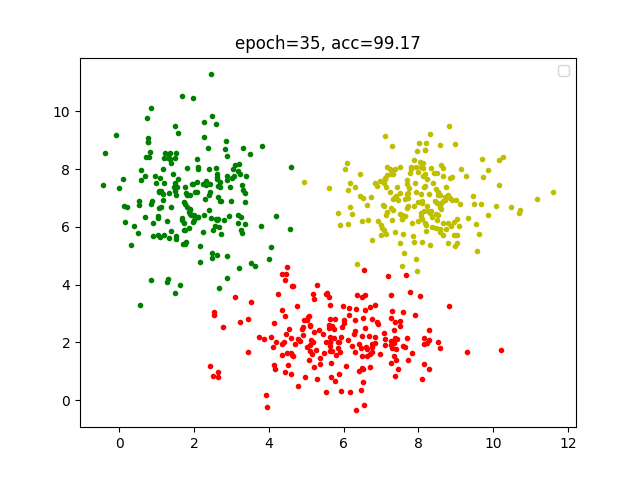
\includegraphics[width=0.7\linewidth]{images/ml_lab3_3.png}
	\caption{}
	\label{fig:mllab33}
\end{figure}

可以看到,在完成$35$轮迭代之后GMM算法收敛,得到最佳的中心点,预测准确率为$99.17\%$。GMM算法收敛速度较快,准确率也比较高。

\subsection{UCI数据集}

我们选用UCI数据集 \href{http://archive.ics.uci.edu/ml/datasets/Iris}{Iris},该数据集共有$150$个数据,类别数为$3$,分别选用k-means和GMM算法进行实验,实验结果表\ref{table:1}所示。

\begin{table}[h]
	\centering
	\begin{tabular}{ccc}
		\textbf{算法} & \textbf{迭代次数} & \textbf{准确率} \\ \hline
		k-means & 6 & 89.33\% \\
		GMM & 61 & 96.67\%
	\end{tabular}
	\caption{}
	\label{table:1}
\end{table}

我们可以看到,在UCI数据集上,GMM算法比k-means算法效果更好,但收敛速度较慢。


\section{结论}

k-means算法较易理解与实现,在简单数据集上效果很好并且收敛较快;GMM的实现复杂,推导繁琐,在各种数据集上都能取得良好的效果,收敛速度较k-means缓慢。


\nocite{*}

\appendix
%\appendixpage
\addappheadtotoc
\section{源代码(带注释)}
\subsection{生成数据}

\lstinputlisting[
style       =   Python,
caption     =   {\bf data.py},
label       =   {data.py}
]{codes/data.py}


\subsection{k-means算法}

\lstinputlisting[
style       =   Python,
caption     =   {\bf kmeans.py},
label       =   {kmeans.py}
]{codes/kmeans.py}


\subsection{GMM算法}

\lstinputlisting[
style       =   Python,
caption     =   {\bf GMM.py},
label       =   {GMM.py}
]{codes/GMM.py}


\subsection{解析UCI数据集}

\lstinputlisting[
style       =   Python,
caption     =   {\bf ucidata.py},
label       =   {ucidata.py}
]{codes/ucidata.py}


\subsection{辅助代码}

\lstinputlisting[
style       =   Python,
caption     =   {\bf utils.py},
label       =   {utils.py}
]{codes/utils.py}


\end{document}
